
\paragraph{Space-Time Duality} 
We now define the set $m(X)\triangleq\{m(x)\ |\ x\in X\}$. We define a dynamical system $(m(X),m\circ c\colon m(X)\rightarrow m(X))$, whose associated set of behaviours is $(m\circ c)_{m(X)}^\infty$.

\begin{figure}[t]
    \centering
    \begin{tikzcd}%[column sep=1.75cm, row sep=1cm]
        (X\times m(X), (c \circ m,m \circ c))
            \arrow[d,swap,"\fst"]
            \arrow[r,swap,"\snd"]
        & (m(X), m \circ c)
            \arrow[d,swap,"m\circ c_{(\cdot)}^\infty"']
        \\ 
        (X,c \circ m)
            \arrow[r,swap,"(c\circ m)_{(\cdot)}^\infty"]
        &  (X^\infty, (\cdot)')
    \end{tikzcd} 
    \caption{Pullback relating $c\circ m$ and $m\circ c$, describing the space-time duality of dynamical systems defined by $\id$-coalgebras.}
\end{figure}

\begin{theorem}[Fundamental Theorem of Latent-Behaviour Analysis]
    \label{theo:Fundamental}
    The semantic map-ping of the $F$-coalgebra $(X,c\circ m\colon X\rightarrow F(X))$ factors through the semantic mapping of the $F$-coalgerba $(m(X),c\colon m(X)\rightarrow F(m(X)))$
    \todo[inline]{This probably needs to use bounded functors.}
\end{theorem}
\begin{proof}
    The Epi-mono factorisation from Universal Coalgebra uses the kernel of homomorphisms as the quotient. Here, we replace it by $\equiv_m$, enforcing bisimilarity between $x$ and $m(x)$. Note that $\equiv_{\id}$ results in normal bisimilarity, because no enforcement takes place.

    The transformation $m\colon X\rightarrow X$ forces the appearances of equivalence classes $\equiv_m\subseteq X\times X$ with respect to $c$, where $x_1\equiv_m x_2$ iff $m(x_1)\sim m(x_2)$, which overrides bisimilarity in $X$ with respect to $c$. The set $X/\equiv_m$ is isomorphic to $m(X)$. In other words, 
\end{proof}

\begin{figure}[t]
    \centering
    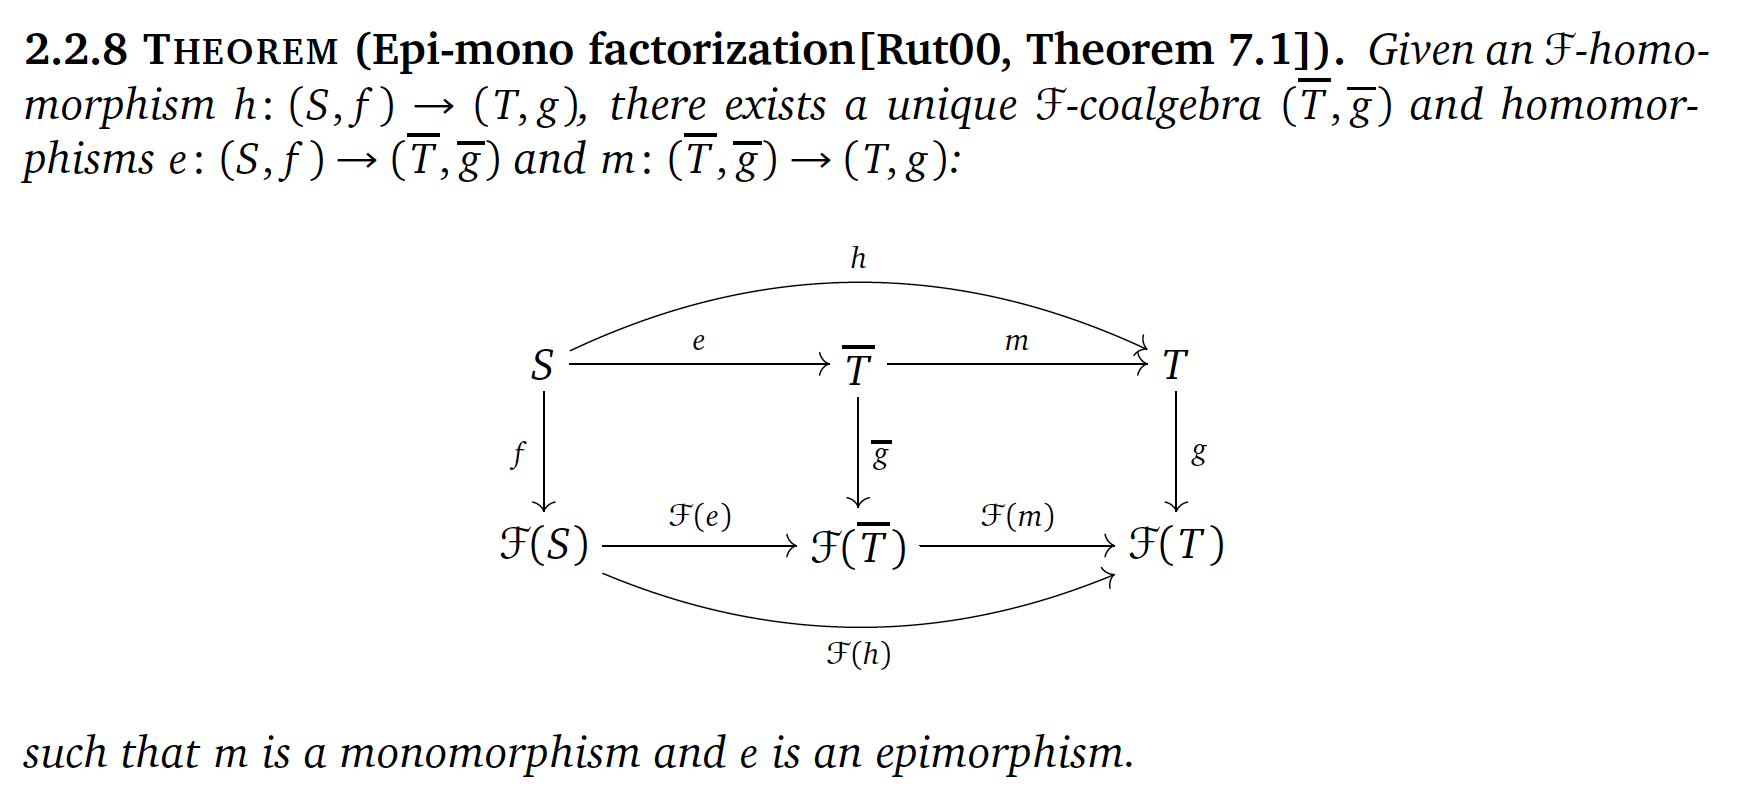
\includegraphics[width=1\textwidth]{Figures/Epi-monofactorisation.png}
    \caption{Reason why the fundamental theorem works.}
    \label{fig:LambdaCurves}
    \end{figure}

\begin{figure}[t]
    \centering
    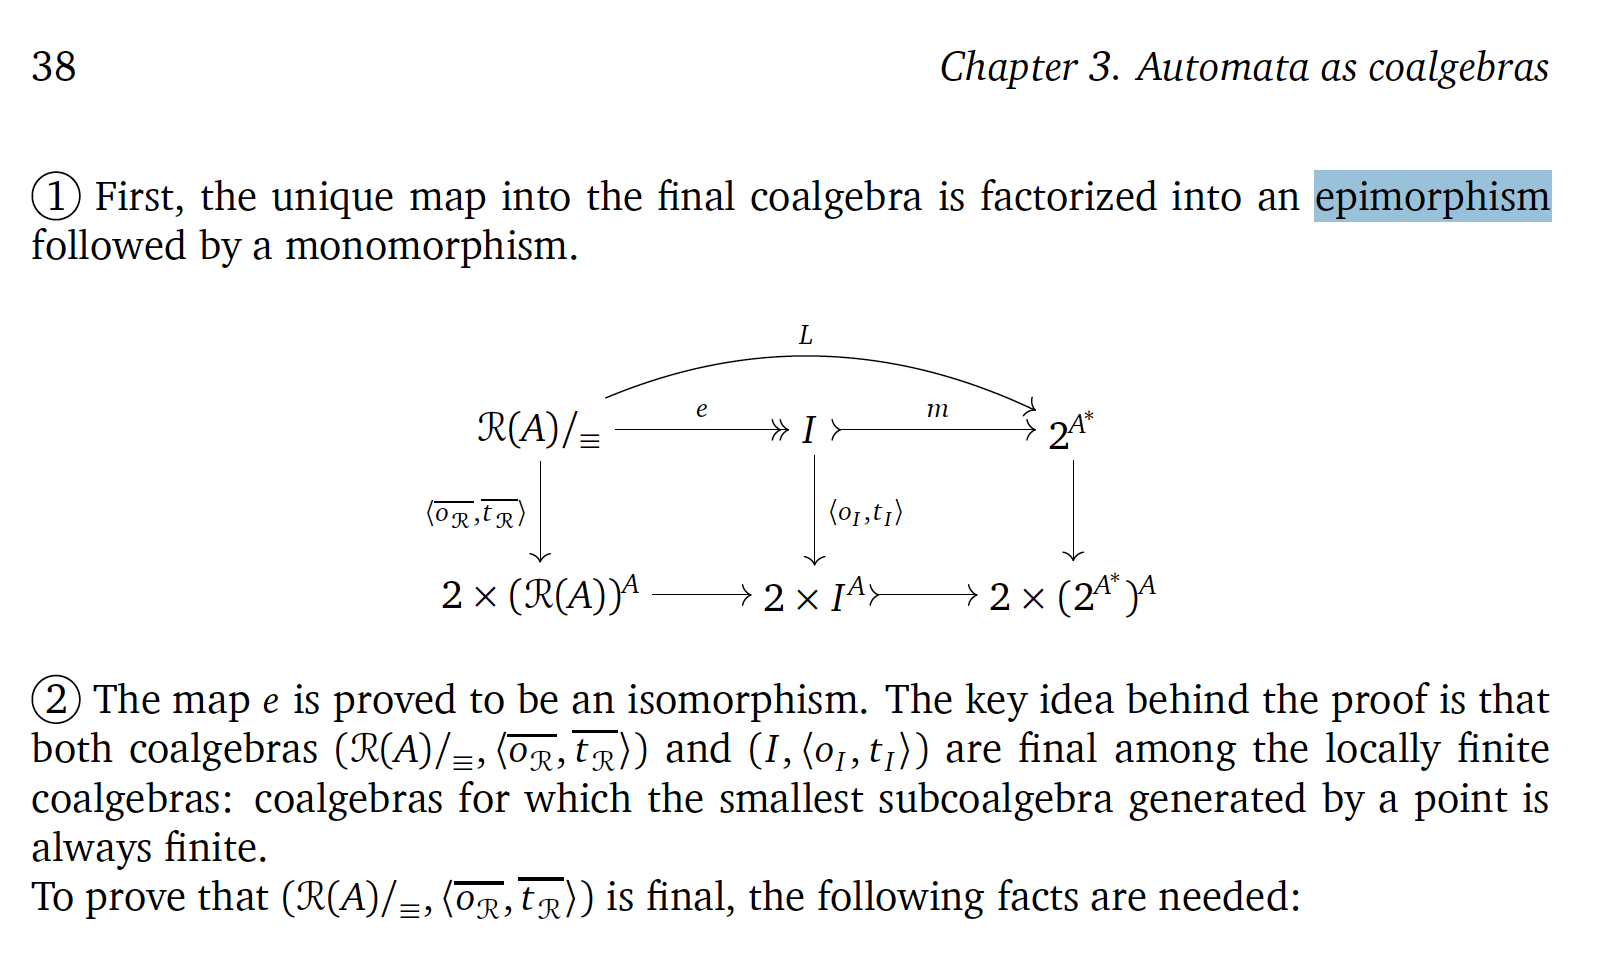
\includegraphics[width=1\textwidth]{Figures/FundamentalTheo.png}
    \caption{Reason why the fundamental theorem works.}
    \label{fig:LambdaCurves}
    \end{figure}

\begin{proposition}[Behavioural Change]
For any dynamical system described by an $F$-coalgebra 
$(X,c\circ m\colon X\rightarrow F(X))$, where $m\colon X\rightarrow X$, and  $c\colon X\rightarrow F(X)$, there exists a \emph{unique} transformation function $\Delta_m\colon \sigma F\rightarrow \sigma F$ which maps $\TheBehaviourOfIn{x}{c}$ to $\TheLatentBehaviourOfIn{x}{c}{m}$, describing the \emph{behavioural change} of $x$, for all $x\in X$.
\end{proposition}
\begin{proof}
    The function $\Delta_{m}\colon \sigma F\rightarrow \sigma F$ is an $F$-coalgebra since $F(\sigma F)\simeq \sigma F$, so it has a behaviour. 
coinductively defined by 
{\color{red}
\todo[inline]{Transform this into a commutative diagram?}
\begin{align*}
    \Delta_{m}(\TheBehaviourOfIn{x}{c}) \sim_{(c \circ m)} (x)\\
    %\Delta_{m}(c^\infty_x)[1]&\triangleq c^\infty_{m(x)}[1]\\
    \Delta_{m}(c^\infty_x)[t+1]&\triangleq \Delta_{m}\left(c^\infty_{(c\circ m)(x)}\right)[t]
\end{align*}
}
\end{proof}

\section{Dynamical Systems of the $\id$ Functor}
% Theorem~\ref{theo:Fundamental} is a far stretch from the fundamental theorem of arithmetic, which states that every natural number can be decomposed into a multiplication of primes, but it follows a similar reasoning. Normally, we ignore this decomposition, so $\delta=c$ and $m=\id$. 
% \todo[inline]{It would be nice to have ``primes" here, and they may exist. They'll probably }



The \emph{fundamental theorem of latent behaviour analysis} implies the existence of unique transformation function $\Delta_m\colon X^\infty\rightarrow X^\infty$ which maps $c_{x}^\infty$ to both $\delta_{x}^\infty$ and $c_{m(x)}^\infty$ for all $x\in X$. The function $\Delta_m$ models the behavioural change induced by $m$ when applied to the $F$-coalgebra $(X,c)$. This unique function $\delta_{x}^\infty$ and $c_{m(x)}^\infty$ is 
coinductively defined by 
% \todo[inline]{BE CAREFUL HOW YOU DEFINE THE INDICES and if you want behaviours to include $x$, in coalgberas that is not very common.}
\begin{align*}
    \Delta_{m}(c^\infty_x)[0]&\triangleq (c \circ m)(x)\\
    %\Delta_{m}(c^\infty_x)[1]&\triangleq c^\infty_{m(x)}[1]\\
    \Delta_{m}(c^\infty_x)[t+1]&\triangleq \Delta_{m}\left(c^\infty_{(c\circ m)(x)}\right)[t]
\end{align*}
This definition compounds the effect of $m$ over time.
% \begin{align}
%     \Delta_m(c_{x}^\infty)\triangleq(m\circ c)_{x}^\infty
% \end{align}
% which is not a very useful definition. However, if $m$ satisfies some linearity properties, then this function $\Delta_m(c_{x}^\infty)$ can be defined (co)inductively.

For example, consider the system $(\mathbb{N},c=(+1))$ and the operator $m=(*3)$. The corresponding definition is $\Delta_{m}$ by
\begin{align*}
    \Delta_{m}(c^\infty_x)[0]&=1\\%(+1)^\infty_{2x}[1]\\
    (\Delta_{m}(c^\infty_x))[t+1]&=\Delta_{m}(c^\infty_{3x+1})[t]
\end{align*}
%This definition compounds the effect of the operator $(*2)$. 
From $(1,2,3,\ldots)=(+1)^\infty_0$, we obtain the sequence $(1,7,13,40,121,\ldots)$. 
% Now, $\Delta_{(*2)}(\omega)[0]=0$. %, so $((+1)\circ (*2))^\infty_0[0]=0$. 
% Next, $\Delta_{(*2)}(((+1)\circ (*2))^\infty_{1})[0]=1$

%$\Delta_{(*2)}(\omega)[t+1]$ since $\omega=(+1)^\infty_{(2*0)+1}$
\begin{definition}
The operator $m$ is \emph{linear with respect to $c$} if and only if
\begin{align}
    (c\circ m)^\infty_x[t]= (m \circ c)^\infty_x[t].
\end{align}    
\end{definition}

%Functorial operators are quite rare. It means that their effects do not compound over time. 
% (Linear operators have a deep relation to bialgebras of the identity functor, where $c\circ m= m\circ c $.)
% The operator $(*2)$ is not linear with respect to $(+1)$, but the operator $+3$ is. $(0,4,8,)$.

Depending on the properties of $m$ and $\Delta_m$, we might infer whether some behavioural property was preserved for all sequences, i.e., if $P(c^\infty_x)$, then $P((c\circ m)^\infty_x)$. For example, for $m=(*3)$, and $c=(+1)$, the sequence is still strictly increasing. 



%We say that thefunction $\Delta^m$ has a solution if it can be written








THe usefulness of latent behaviour analysis is that you can decompose a behaviour-defining into several components. Each of those components 



\todo[inline]{Latent coalgebras are coalgebras with the state space deformed.}
\todo[inline]{THESE DIAGRAMS ARE WRONG. THE BEH OF C CANNOT APPEAR LIKE THISOR YOU CAN GO VIA M to the end of c}
\end{definition}
\begin{figure}
    \centering
    \begin{tikzcd}[column sep=large]
        \sigma F
            \arrow[d, "\simeq","\omega"'] 
        &X
            \arrow[r, "m"]
            %\arrow[rd, "c\circ m", red]
            \arrow[l, dotted, swap,"\TheBehaviourOf{\cdot}_{c\circ m}"]
        &X 
            \arrow[r, dotted, "\TheBehaviourOf{\cdot}_c"] 
            \arrow[d, "c"] 
        & \sigma F 
            \arrow[d, "\simeq","\omega"'] 
        \\
        F(\sigma F)
        &
        &F(X) 
            \arrow[r, dotted, "F(\TheBehaviourOf{\cdot}_c)"]
            \arrow[ll, dotted, swap,"F(\TheBehaviourOf{\cdot}_{c\circ m})"]     
        &F(\sigma F)
    \end{tikzcd}
    \caption{$(X,c\circ m)$ is an $F$-coalgebra, so it has a unique $F$-homomorphism to the final $F$-coalgebra $(\sigma F, \omega)$. Geometrically, $m$ is a transformation of the state space, so some preserve certain structural properties (e.g. a permutation) while others do not (e.g. a collapsing function to some fixed $x$).}
\end{figure}
\begin{figure}
    \centering
    \begin{tikzcd}[column sep=large]
        \sigma F
            \arrow[d, "\simeq","\omega"'] 
        &&X
            \arrow[r, "m"]
            \arrow[d, "b\circ c\circ m"] 
            %\arrow[rd, "c\circ m", red]
            \arrow[ll, dotted, swap,"\TheBehaviourOf{\cdot}_{b\circ c\circ m}"]
        &X 
            \arrow[rr, dotted, "\TheBehaviourOf{\cdot}_c"] 
            \arrow[d, "c"] 
        && \sigma F 
            \arrow[d, "\simeq","\omega"'] 
        \\
        F(\sigma F) 
        &&F(X) \arrow[ll, dotted, swap,"F(\TheBehaviourOf{\cdot}_{b\circ c\circ m})"]
        &F(X) 
            \arrow[rr, dotted, "F(\TheBehaviourOf{\cdot}_c)"]
            \arrow[l, "b"]     
        &&F(\sigma F)
    \end{tikzcd}
    \caption{Latency using both $m$ and $b$ to reveal latent behaviours: $(X,b\circ c\circ m)$ is still an $F$-coalgebra, so it has a unique $F$-homomorphism to the final $F$-coalgebra $(\sigma F, \omega)$. Metaphorically, consider the function $c$ as a causal model which transforms the cause $x$ into the consequence $c(x)$; the transformation $m$ corresponds to a change of cause, while a transformation $b$ corresponds to a change of consequence. In a more concrete example, assume that we are grading a test, and $c$ is the grading rules. The value $c(x)$ is the grade assigned to the answers $x$. A transformation $m$ would correspond to changing the answers before grading, while a transformation $b$ corresponds to changing the grade after the answers have been graded. Now, if $F(X)$ is the The transformation $b$ needs not respect the properties of $c$, since it is applied after it. Thus, it would be possible to change the grade through $b$ to some value that is impossible to obtain by any possible combination of answers (i.e. for every $m$ that changes answers).}
\end{figure}
\begin{figure}
    \centering
    \begin{tikzcd}[column sep=large]
        \sigma F
            \arrow[d, "\simeq","\omega"'] 
        &X
            \arrow[r, "m"]
            %\arrow[rd, "c\circ m", red]
            \arrow[l, dotted, swap,"\TheBehaviourOf{\cdot}_{c\circ m}"]
        &X 
            \arrow[r, dotted, "\TheBehaviourOf{\cdot}_c"] 
            \arrow[d, "c"] 
        & \sigma F 
            \arrow[d, "\simeq","\omega"'] 
        \\
        F(\sigma F)
        &
        &F(X) 
            \arrow[r, dotted, "F(\TheBehaviourOf{\cdot}_c)"]
            \arrow[ll, dotted, swap,"F(\TheBehaviourOf{\cdot}_{c\circ m})"]     
        &F(\sigma F)
    \end{tikzcd}
    \caption{$(X,T(X)\xrightarrow{c\circ a}F(X))$ is an $FT$-coalgebra, (not quite a bialgebra, but it could be). $T(X)$ defines specifications for $X$, so we could mutate those instead of $X$ directly. This is what the paper by Harrison and Goldstein does \cite{DoJudgeATestByItsCover}}
\end{figure}


{\color{red}The deformation $b$ is not that interesting because it is too flexible. If $F=\id$ then $t$ has the same type as $s$ and they compose, so we can approximate $t.c.s$ with $c.s'$, where $s'=s.t$. If $F(X)$ has only one component, then $t=const \phi$ forces the system to have the behaviour that the attacker wants. More precisely, it can reveal any $F$-coalgebra for that carrier set. The balance would be to allow the attacker of $t$ to influence only a set of components in $F(X)$, just like we do with $s$. Consider the $F$-coalgebras of $()$ for the functor $2x\id^2$; there are only two: $c_0(())=(False,const ())$ and $c_1(())=(True,const ())$. Using state transformations we cannot reveal new behaviours given $c_0$ or $c_1$, but with with behaviour transformations we can: $t=(\texttt{not},\id)$ causes $t.c_0=c_1$ and $t.c_1=c_0$ so you can strictly do more. The question is, do we need more? 

Poetically, $m$ corresponds to a deformation of space, and $b$ corresponds to a deformation of causality.
}

\begin{example}
\label{ex:LatentBehaviour}
Consider the functor $G=2\times \texttt{id}^2$ and a $G$-coalgebra $\mathbb{X}=(2\times2,(\gamma,\delta))$ 
\todo[inline]{Match with the right automaton}
. We define said $G$-coalgebra $\mathbb{X}$ by
\begin{align}
\gamma(x,y)&\triangleq x \land y;\\
\delta(x,y)(i)&\triangleq(i,x).
\end{align}
Figure~\ref{fig:ExampleLatent} shows the deterministic finite automaton corresponding to this $G$-coalgebra; the coalgebra is not minimal, because the states $(0,0)$ and $(0,1)$ are bisimilar.
% \begin{figure}[t]
% \centering
% \begin{tikzpicture}
% \node[state] (00) {$(0,0)$};
% \node[state, below right of=00] (01) {$(0,1)$};
% \node[state, above right  of=00] (10) {$(1,0)$};
% \node[state, accepting, below right of=10] (11) {$(1,1)$};
% \draw (00) edge[bend left, above] node{1} (10)
% (00) edge[loop above] node{0} (00)
% (01) edge[bend left, above] node[left]{1} (10)
% (01) edge[bend left, above] node{0} (00)
% (10) edge[bend left, above] node{1} (11)
% (10) edge[bend left, above] node[right]{0} (01)
% (11) edge[loop above] node{1} (11)
% (11) edge[bend left, above] node{0} (01)
% ;\end{tikzpicture}
% \caption{Corresponding automaton to the $G-$coalgebra described in Example~\ref{ex:LatentBehaviour}.}
% \label{fig:ExampleLatent}
% \end{figure}

This $G$-coalgebra has 256 transformations, given by the $4^4$ endofunctions in $X$. We use these transformations to reveal latent behaviours.%, and every consistent transformation $m$ satisfies $m(0,0)~m(0,1)$. 
\todo[inline]{You can probably graph this with a 3 dimensional graph like a vector field whose axises are input, state, and output. We could use four dimensions so that state is 2-dimensional}
% We present the automata that correspond to latent $G-$coalgebras in Figures~\ref{fig:3.2}--\ref{fig:3.28}. Note that many of these latent coalgebras are not minimal, and many display the same behaviours.

% From 27 endofuctions and three intended behaviours, we can derive the 24 latent behaviours presented in Table~\ref{tab:ExampleLatentBehaviours} as regular expressions. 
{\color{red}
\todo[inline]{Rewrite this!!!}
The existence of latent behaviours opens a new possibility for system repurposing: if we wanted the system to recognise the language $(0+1)^*1$ (i.e., the language of sequences that end in 1), we could mutate our original system using a transformation where $0\mapsto0, 1\mapsto2$ and $2\mapsto2$ (shown in Figure~\ref{fig:3.10}), whilst preserving $0$ as the initial state. Nevertheless, if providing the transformation is within the capabilities of an adversary, it would also mean that they can repurpose our system as well. 
}


\begin{figure}[t]
\centering
\begin{tikzpicture}
    \node[state] (00) {$(0,0)$};
    \node[state, below right of=00] (01) {$(0,1)$};
    \node[state, above right  of=00] (10) {$(1,0)$};
    \node[state, accepting, below right of=10] (11) {$(1,1)$};
    \draw (00) edge[bend left, above] node{1} (10)
    (00) edge[loop above] node{0} (00)
    (01) edge[bend left, above] node{1} (11)
    (01) edge[loop above] node{0} (01)
    (10) edge[loop above] node{1} (10)
    (10) edge[bend left, above] node{0} (00)
    (11) edge[loop above] node{1} (11)
    (11) edge[bend left, above] node{0} (01)
    ;\end{tikzpicture}
\caption{Corresponding automaton to the latent $G-$coalgebra under transformation $(a,b)\mapsto(b,a)$. This transformation is not consistent, since $(0,0)\sim (0,1)$ in the original $F$-coalgebra, but $(0,0)$ and $(1,0)$ are no longer bisimilar}% described in Example~\ref{ex:LatentBehaviour}.}
\label{fig:ExampleInconsistentLatent}
\end{figure}

\begin{figure}[t]
\centering
\begin{tikzpicture}
    \node[state] (00) {$(0,0)$};
    \node[state, below right of=00] (01) {$(0,1)$};
    \node[state, accepting, above right  of=00] (10) {$(1,0)$};
    \node[state, accepting, below right of=10] (11) {$(1,1)$};
    \draw (00) edge[bend left, above] node{1} (10)
    (00) edge[loop above] node{0} (00)
    (01) edge[bend left, above] node{1} (10)
    (01) edge[bend left, above] node{0} (00)
    (10) edge[bend left, above] node{1} (11)
    (10) edge[bend left, above] node{0} (01)
    (11) edge[loop above] node{1} (11)
    (11) edge[bend left, above] node{0} (01)
    ;\end{tikzpicture}
\caption{Corresponding automaton to the latent $G-$coalgebra under transformation $(0,x)\mapsto (0,0)$ and $(1,x)\mapsto (1,1)$. This transformation is consistent, and reveals a new behaviour from the state $(0,0)$, more precisely, the language $(0,1)^*1$ of sequences that end in $1$.}% described in Example~\ref{ex:LatentBehaviour}.}
\label{fig:ExampleConsistentLatent}
\end{figure} 
    
% \begin{table}[t]
% \centering
% \begin{tabular}{|l | l | }
% \hline
% $\rho_{\ref{fig:3.2}.0}$ &  $\emptyset$   \\
% $\rho_{\ref{fig:3.4}.2}$ &  $1^*$ \\
% $\rho_{\ref{fig:3.7}.0}$ &  $(0+1)^*111^*$\\%$(0+10+111^*0)^*111^*$ \\
% $\rho_{\ref{fig:3.7}.1}$ &  $\rho_{\ref{fig:3.7}.0}+1$ \\
% $\rho_{\ref{fig:3.7}.2}$ &  $\rho_{\ref{fig:3.7}.0}+1+\varepsilon$ \\
% $\rho_{\ref{fig:3.8}.1}$ &  $(00^*1+10^*1)^*$ \\
% $\rho_{\ref{fig:3.8}.0}$ &  $0^*1\rho_{\ref{fig:3.8}.1}$ \\
% $\rho_{\ref{fig:3.9}.2}$& $(0+1)^*01$\\
% $\rho_{\ref{fig:3.9}.0}$&   $\rho_{\ref{fig:3.9}.2}+1$\\
% $\rho_{\ref{fig:3.9}.1}$&   $\rho_{\ref{fig:3.9}.2}+1+\varepsilon$\\
% $\rho_{\ref{fig:3.10}.0}$ &  $(0+1)^*1$ \\
% $\rho_{\ref{fig:3.10}.1}$ &  $\rho_{\ref{fig:3.10}.0}+\varepsilon$ \\
% $\rho_{\ref{fig:3.13}.1}$ &  $1^*0\rho_{\ref{fig:3.10}.0}$ \\
% $\rho_{\ref{fig:3.17}.0}$ &  $(0+10+(11)^+(0+10))^*(11)^+$ \\
% $\rho_{\ref{fig:3.17}.1}$ &  $(11)^*+(0+10)\rho_{\ref{fig:3.17}.0}$ \\
% $\rho_{\ref{fig:3.17}.2}$ &  $0\rho_{\ref{fig:3.17}.0}+1\rho_{\ref{fig:3.17}.1}$ \\
% $\rho_{\ref{fig:3.18}.0}$ &  $\varepsilon$ \\
% $\rho_{\ref{fig:3.20}.1}$ &  $(0+1)^*0$ \\
% $\rho_{\ref{fig:3.20}.0}$ &  $\rho_{\ref{fig:3.20}.1}+\varepsilon$ \\
% $\rho_{\ref{fig:3.22}.0}$ &  $(1+0)^*$ \\
% $\rho_{\ref{fig:3.22}.1}$ &  $1^*0(1+0)^*$ \\
% $\rho_{\ref{fig:3.25}.1}$ &  $1(1+0)^*+0(1+0)^*$ \\
% $\rho_{\ref{fig:3.26}.0}$ &  $(0+10+11)^*$ \\
% $\rho_{\ref{fig:3.26}.2}$ &  $(0+1)\rho_{\ref{fig:3.26}.0}$\\
% \hline
% \end{tabular}
% \caption{Latent behaviours for all transformations for the coalgebra that recognises $(0+1)^*11$. }
% \label{tab:ExampleLatentBehaviours}
% \end{table}

% %$\rho_{\ref{fig:3.8}.0}$ &  $$ \\
% %$\rho_{\ref{fig:3.8}.1}$ &  $$ \\
% %$\rho_{\ref{fig:3.8}.2}$ &  $$ \\
% %------------------------------------------------------------------------------------------------------------------------
% \begin{figure}[t]
% \centering
% \begin{tikzpicture}
% \node[state] (q1) {$0$};
% \node[state, right of=q1] (q2) {$1$};
% \node[state, right of=q2] (q3) {$2$};
% \draw (q1) edge[loop above] node{0} (q1)
% (q1) edge[bend left, above] node{1} (q2)
% (q2) edge[bend left, above] node{0} (q1)
% (q2) edge[loop above] node{1} (q2)
% (q3) edge[bend left, above] node{1} (q2)
% (q3) edge[bend left, below] node{0} (q1);
% \end{tikzpicture}
% \caption{Latent coalgebra under graph $G(m)=\set{(0,0),(1,0),(2,0)}$. $\TheLatentBehaviourOf{0}{m}=\TheLatentBehaviourOf{1}{m}=\TheLatentBehaviourOf{2}{m}=\emptyset$ }
% \label{fig:3.2}

% \begin{tikzpicture}
% \node[state] (q1) {$0$};
% \node[state, right of=q1] (q2) {$1$};
% \node[state, right of=q2] (q3) {$2$};
% \draw (q1) edge[loop above] node{0} (q1)
% (q1) edge[bend left, above] node{1} (q2)
% (q2) edge[bend left, above] node{0} (q1)
% (q2) edge[loop above] node{1} (q2)
% (q3) edge[loop above] node{1} (q3)
% (q3) edge[bend left, below] node{0} (q1);
% \end{tikzpicture}
% \caption{Latent coalgebra under graph $G(m)=\set{(0,0),(1,0),(2,1)}$. $\TheLatentBehaviourOf{0}{m}=\TheLatentBehaviourOf{1}{m}=\TheLatentBehaviourOf{2}{m}=\emptyset$}
% \label{fig:3.3}

% \begin{tikzpicture}
% \node[state] (q1) {$0$};
% \node[state, right of=q1] (q2) {$1$};
% \node[state, accepting, right of=q2] (q3) {$2$};
% \draw (q1) edge[loop above] node{0} (q1)
% (q1) edge[bend left, above] node{1} (q2)
% (q2) edge[bend left, above] node{0} (q1)
% (q2) edge[loop above] node{1} (q2)
% (q3) edge[loop above] node{1} (q3)
% (q3) edge[bend left, below] node{0} (q1);
% \end{tikzpicture}
% \caption{Latent coalgebra under graph $G(m)=\set{(0,0),(1,0),(2,2)}$. $\TheLatentBehaviourOf{0}{m}=\TheLatentBehaviourOf{1}{m}=\emptyset$, $\TheLatentBehaviourOf{2}{m}=1^*$}
% \label{fig:3.4}
% \end{figure}

% \begin{figure}[t]
% \captionsetup{singlelinecheck=off}
% \centering
% \begin{tikzpicture}
% \node[state] (q1) {$0$};
% \node[state, right of=q1] (q2) {$1$};
% \node[state, right of=q2] (q3) {$2$};
% \draw (q1) edge[loop above] node{0} (q1)
% (q1) edge[bend left, above] node{1} (q2)
% (q2) edge[bend left, above] node{0} (q1)
% (q2) edge[bend left, above] node{1} (q3)
% (q3) edge[bend left, above] node{1} (q2)
% (q3) edge[bend left, below] node{0} (q1);
% \end{tikzpicture}
% \caption{Latent coalgebra under graph $G(m)=\set{(0,0),(1,1),(2,0)}$ . $\TheLatentBehaviourOf{0}{m}=\TheLatentBehaviourOf{1}{m}=\TheLatentBehaviourOf{2}{m}=\emptyset$}

% \begin{tikzpicture}
% \node[state] (q1) {$0$};
% \node[state, right of=q1] (q2) {$1$};
% \node[state, right of=q2] (q3) {$2$};
% \draw (q1) edge[loop above] node{0} (q1)
% (q1) edge[bend left, above] node{1} (q2)
% (q2) edge[bend left, above] node{0} (q1)
% (q2) edge[bend left, above] node{1} (q3)
% (q3) edge[loop above] node{1} (q3)
% (q3) edge[bend left, below] node{0} (q1);
% \end{tikzpicture}
% \caption{Latent coalgebra under graph $G(m)=\set{(0,0),(1,1),(2,1)}$ . $\TheLatentBehaviourOf{0}{m}=\TheLatentBehaviourOf{1}{m}=\TheLatentBehaviourOf{2}{m}=\emptyset$}

% \begin{tikzpicture}
% \node[state] (q1) {$0$};
% \node[state, right of=q1] (q2) {$1$};
% \node[state,accepting, right of=q2] (q3) {$2$};
% \draw (q1) edge[loop above] node{0} (q1)
% (q1) edge[bend left, above] node{1} (q2)
% (q2) edge[bend left, above] node{0} (q1)
% (q2) edge[bend left, above] node{1} (q3)
% (q3) edge[loop above] node{1} (q3)
% (q3) edge[bend left, below] node{0} (q1);
% \end{tikzpicture}
% \caption{Latent coalgebra under graph $G(m)=\set{(0,0),(1,1),(2,2)}$ (i.e. $m=\texttt{id}$). Latent behaviours under $m$ are the original behaviours: 
% \protect\begin{align*}
% 	\TheLatentBehaviourOf{0}{m}&=(0+1)^*111^*, \\
% 	\TheLatentBehaviourOf{1}{m}&=1+\TheLatentBehaviourOf{0}{m}\\
% 	\TheLatentBehaviourOf{2}{m}&=\varepsilon + 1+ \TheLatentBehaviourOf{0}{m}
% \protect\end{align*}
% }
% \label{fig:3.7}
% \end{figure}



% \begin{figure}[t]
% \captionsetup{singlelinecheck=off}
% \centering
% \begin{tikzpicture}
% \node[state] (q1) {$0$};
% \node[state,accepting, right of=q1] (q2) {$1$};
% \node[state, right of=q2] (q3) {$2$};
% \draw (q1) edge[loop above] node{0} (q1)
% (q1) edge[bend left, above] node{1} (q2)
% (q2) edge[bend left, above] node{0} (q1)
% (q2) edge[bend left, above] node{1} (q3)
% (q3) edge[bend left, above] node{1} (q2)
% (q3) edge[bend left, below] node{0} (q1);
% \end{tikzpicture}
% \caption{Latent coalgebra under graph $G(m)=\set{(0,0),(1,2),(2,0)}$. 
% \protect\begin{align*}
% \TheLatentBehaviourOf{0}{m}&=\TheLatentBehaviourOf{2}{m}=0^*1\TheLatentBehaviourOf{1}{m},\\
% \TheLatentBehaviourOf{1}{m}&=(00^*1+10^*1)^*
% \protect\end{align*}
% \label{fig:3.8}
% }

% \begin{tikzpicture}
% \node[state] (q1) {$0$};
% \node[state,accepting, right of=q1] (q2) {$1$};
% \node[state, right of=q2] (q3) {$2$};
% \draw (q1) edge[loop above] node{0} (q1)
% (q1) edge[bend left, above] node{1} (q2)
% (q2) edge[bend left, above] node{0} (q1)
% (q2) edge[bend left, above] node{1} (q3)
% (q3) edge[loop above] node{1} (q3)
% (q3) edge[bend left, below] node{0} (q1);
% \end{tikzpicture}
% \caption{Latent coalgebra under graph $G(m)=\set{(0,0),(1,2),(2,1)}$.
% \protect\begin{align*}
% \TheLatentBehaviourOf{0}{m}&=1+\TheLatentBehaviourOf{2}{m},\\
% \TheLatentBehaviourOf{1}{m}&=\varepsilon+1+\TheLatentBehaviourOf{2}{m},\\
% \TheLatentBehaviourOf{2}{m}&=(0+1)^*01
% \protect\end{align*}
% \label{fig:3.9}
% }

% \begin{tikzpicture}
% \node[state] (q1) {$0$};
% \node[state,accepting, right of=q1] (q2) {$1$};
% \node[state, accepting,right of=q2] (q3) {$2$};
% \draw (q1) edge[loop above] node{0} (q1)
% (q1) edge[bend left, above] node{1} (q2)
% (q2) edge[bend left, above] node{0} (q1)
% (q2) edge[bend left, above] node{1} (q3)
% (q3) edge[loop above] node{1} (q3)
% (q3) edge[bend left, below] node{0} (q1);
% \end{tikzpicture}
% \caption{Latent coalgebra under graph $G(m)=\set{(0,0),(1,2),(2,2)}$.
% \protect\begin{align*}
% \TheLatentBehaviourOf{0}{m}&=(0+1)^*1,\\ 
% \TheLatentBehaviourOf{1}{m}&=\TheLatentBehaviourOf{2}{m}=\varepsilon + \TheLatentBehaviourOf{0}{m}
% \protect\end{align*}
% \label{fig:3.10}
% }
% \end{figure}

% \begin{figure}[t]
% \captionsetup{singlelinecheck=off}
% \centering
% \begin{tikzpicture}
% \node[state] (q1) {$0$};
% \node[state, right of=q1] (q2) {$1$};
% \node[state, right of=q2] (q3) {$2$};
% \draw (q1) edge[loop above] node{0} (q1)
% (q1) edge[bend left, above] node{1} (q3)
% (q2) edge[bend left, above] node{0} (q1)
% (q2) edge[loop right] node{1} (q2)
% (q3) edge[bend left, above] node{1} (q2)
% (q3) edge[bend left, below] node{0} (q1);
% \end{tikzpicture}
% \caption{Latent coalgebra under graph $G(m)=\set{(0,1),(1,0),(2,0)}$. $\TheLatentBehaviourOf{0}{m}=
% \TheLatentBehaviourOf{1}{m}=\TheLatentBehaviourOf{2}{m}=\emptyset$}

% \begin{tikzpicture}
% \node[state] (q1) {$0$};
% \node[state, right of=q1] (q2) {$1$};
% \node[state, right of=q2] (q3) {$2$};
% \draw (q1) edge[loop above] node{0} (q1)
% (q1) edge[bend left, above] node{1} (q3)
% (q2) edge[bend left, above] node{0} (q1)
% (q2) edge[loop right] node{1} (q2)
% (q3) edge[loop above] node{1} (q3)
% (q3) edge[bend left, below] node{0} (q1);
% \end{tikzpicture}
% \caption{Latent coalgebra under graph $G(m)=\set{(0,1),(1,0),(2,1)}$. $\TheLatentBehaviourOf{0}{m}=
% \TheLatentBehaviourOf{1}{m}=\TheLatentBehaviourOf{2}{m}=\emptyset$}


% \begin{tikzpicture}
% \node[state] (q1) {$0$};
% \node[state, right of=q1] (q2) {$1$};
% \node[state,accepting, right of=q2] (q3) {$2$};
% \draw (q1) edge[loop above] node{0} (q1)
% (q1) edge[bend left, above] node{1} (q3)
% (q2) edge[bend left, above] node{0} (q1)
% (q2) edge[loop right] node{1} (q2)
% (q3) edge[loop above] node{1} (q3)
% (q3) edge[bend left, below] node{0} (q1);
% \end{tikzpicture}
% \caption{Latent coalgebra under graph $G(m)=\set{(0,1),(1,0),(2,2)}$. 
% \protect\begin{align*}
% \TheLatentBehaviourOf{0}{m}&=(0+1)^*1,\\ 
% \TheLatentBehaviourOf{1}{m}&=1^*0\TheLatentBehaviourOf{0}{m},\\
% \TheLatentBehaviourOf{2}{m}&=\varepsilon+\TheLatentBehaviourOf{0}{m}
% %\TheLatentBehaviourOf{2}{m}&=1^*+\TheLatentBehaviourOf{1}{m}
% \protect\end{align*}
% }
% \label{fig:3.13}
% \end{figure}

% \begin{figure}[t]
% \captionsetup{singlelinecheck=off}
% \centering
% \begin{tikzpicture}
% \node[state] (q1) {$0$};
% \node[state, right of=q1] (q2) {$1$};
% \node[state, right of=q2] (q3) {$2$};
% \draw (q1) edge[loop above] node{0} (q1)
% (q1) edge[bend left, above] node{1} (q3)
% (q2) edge[bend left, above] node{0} (q1)
% (q2) edge[bend left, above] node{1} (q3)
% (q3) edge[bend left, above] node{1} (q2)
% (q3) edge[bend left, below] node{0} (q1);
% \end{tikzpicture}
% \caption{Latent coalgebra under graph $G(m)=\set{(0,1),(1,1),(2,0)}$. $\TheLatentBehaviourOf{0}{m}=
% \TheLatentBehaviourOf{1}{m}=\TheLatentBehaviourOf{2}{m}=\emptyset$}


% \begin{tikzpicture}
% \node[state] (q1) {$0$};
% \node[state, right of=q1] (q2) {$1$};
% \node[state, right of=q2] (q3) {$2$};
% \draw (q1) edge[loop above] node{0} (q1)
% (q1) edge[bend left, above] node{1} (q3)
% (q2) edge[bend left, above] node{0} (q1)
% (q2) edge[bend left, above] node{1} (q3)
% (q3) edge[loop above] node{1} (q3)
% (q3) edge[bend left, below] node{0} (q1);
% \end{tikzpicture}
% \caption{Latent coalgebra under graph $G(m)=\set{(0,1),(1,1),(2,1)}$. $\TheLatentBehaviourOf{0}{m}=
% \TheLatentBehaviourOf{1}{m}=\TheLatentBehaviourOf{2}{m}=\emptyset$}


% \begin{tikzpicture}
% \node[state] (q1) {$0$};
% \node[state, right of=q1] (q2) {$1$};
% \node[state, accepting, right of=q2] (q3) {$2$};
% \draw (q1) edge[loop above] node{0} (q1)
% (q1) edge[bend left, above] node{1} (q3)
% (q2) edge[bend left, above] node{0} (q1)
% (q2) edge[bend left, above] node{1} (q3)
% (q3) edge[loop above] node{1} (q3)
% (q3) edge[bend left, below] node{0} (q1);
% \end{tikzpicture}
% \caption{Latent coalgebra under graph $G(m)=\set{(0,1),(1,1),(2,2)}$.
% \protect\begin{align*}
% \TheLatentBehaviourOf{0}{m}&=\TheLatentBehaviourOf{1}{m}=(0+1)^*1,\\ 
% \TheLatentBehaviourOf{2}{m}&=\TheLatentBehaviourOf{0}{m}+\varepsilon
% \protect\end{align*}
% }
% \end{figure}

% \begin{figure}[t]
% \centering
% \captionsetup{singlelinecheck=off}
% \begin{tikzpicture}
% \node[state] (q1) {$0$};
% \node[state,accepting, right of=q1] (q2) {$1$};
% \node[state, right of=q2] (q3) {$2$}; 
% \draw (q1) edge[loop above] node{0} (q1)
% (q1) edge[bend left, above] node{1} (q3)
% (q2) edge[bend left, above] node{0} (q1)
% (q2) edge[bend left, above] node{1} (q3)
% (q3) edge[bend left, above] node{1} (q2)
% (q3) edge[bend left, below] node{0} (q1);
% \end{tikzpicture}
% \caption{Latent coalgebra under graph $G(m)=\set{(0,1),(1,2),(2,0)}$.
% \protect\begin{align*}
% \TheLatentBehaviourOf{0}{m}&=(0+10+(11)^+(0+10))^*(11)^+ \\ %(0+1(0+1(11)^*(0+10)))^*11(11)^* ,\\ 
% \TheLatentBehaviourOf{1}{m}&=(11)^*+(0+10)\TheLatentBehaviourOf{0}{m},\\
% \TheLatentBehaviourOf{2}{m}&=0\TheLatentBehaviourOf{0}{m}+1\TheLatentBehaviourOf{1}{m}
% \protect\end{align*}
% \label{fig:3.17}
% }

% \begin{tikzpicture}
% \node[state] (q1) {$0$};
% \node[state,accepting, right of=q1] (q2) {$1$};
% \node[state, right of=q2] (q3) {$2$};
% \draw (q1) edge[loop above] node{0} (q1)
% (q1) edge[bend left, above] node{1} (q3)
% (q2) edge[bend left, above] node{0} (q1)
% (q2) edge[bend left, above] node{1} (q3)
% (q3) edge[loop above] node{1} (q3)
% (q3) edge[bend left, below] node{0} (q1);
% \end{tikzpicture}
% \caption{Latent coalgebra under graph $G(m)=\set{(0,1),(1,2),(2,1)}$.
% \protect\begin{align*}
% \TheLatentBehaviourOf{0}{m}&=\TheLatentBehaviourOf{2}{m}=\emptyset,\\ 
% \TheLatentBehaviourOf{1}{m}&=\varepsilon
% \protect\end{align*}
% \label{fig:3.18}
% }

% \begin{tikzpicture}
% \node[state] (q1) {$0$};
% \node[state,accepting, right of=q1] (q2) {$1$};
% \node[state, accepting, right of=q2] (q3) {$2$};
% \draw (q1) edge[loop above] node{0} (q1)
% (q1) edge[bend left, above] node{1} (q3)
% (q2) edge[bend left, above] node{0} (q1)
% (q2) edge[bend left, above] node{1} (q3)
% (q3) edge[loop above] node{1} (q3)
% (q3) edge[bend left, below] node{0} (q1);
% \end{tikzpicture}
% \caption{Latent coalgebra under graph $G(m)=\set{(0,1),(1,2),(2,2)}$.
% \protect\begin{align*}
% \TheLatentBehaviourOf{0}{m}&=(0+1)^*1,\\
% \TheLatentBehaviourOf{1}{m}&=\TheLatentBehaviourOf{2}{m}=\varepsilon+\TheLatentBehaviourOf{0}{m}
% \protect\end{align*}
% }
% \end{figure}

% \begin{figure}[t]
% \captionsetup{singlelinecheck=off}
% \centering
% \begin{tikzpicture}
% \node[state, accepting] (q1) {$0$};
% \node[state, right of=q1] (q2) {$1$};
% \node[state, right of=q2] (q3) {$2$};
% \draw (q1) edge[loop above] node{0} (q1)
% (q1) edge[bend left, above] node{1} (q3)
% (q2) edge[bend left, above] node{0} (q1)
% (q2) edge[loop right] node{1} (q2)
% (q3) edge[bend left, above] node{1} (q2)
% (q3) edge[bend left, below] node{0} (q1);
% \end{tikzpicture}
% \caption{Latent coalgebra under graph $G(m)=\set{(0,2),(1,0),(2,0)}$. 
% \protect\begin{align*}
% \TheLatentBehaviourOf{0}{m}&=(0+1)^*0+\varepsilon ,\\ 
% \TheLatentBehaviourOf{1}{m}&=(0+1)^*0
% \protect\end{align*} 
% \label{fig:3.20}
% }

% \begin{tikzpicture}
% \node[state, accepting] (q1) {$0$};
% \node[state, right of=q1] (q2) {$1$};
% \node[state, right of=q2] (q3) {$2$};
% \draw (q1) edge[loop above] node{0} (q1)
% (q1) edge[bend left, above] node{1} (q3)
% (q2) edge[bend left, above] node{0} (q1)
% (q2) edge[loop right] node{1} (q2)
% (q3) edge[loop above] node{1} (q3)
% (q3) edge[bend left, below] node{0} (q1);
% \end{tikzpicture}
% \caption{Latent coalgebra under graph $G(m)=\set{(0,2),(1,0),(2,1)}$.
% \protect\begin{align*}
% \TheLatentBehaviourOf{0}{m}&=(0+1)^*0+\varepsilon ,\\ 
% \TheLatentBehaviourOf{1}{m}&=(0+1)^*0
% \protect\end{align*}
% }

% \begin{tikzpicture}
% \node[state, accepting] (q1) {$0$};
% \node[state, right of=q1] (q2) {$1$};
% \node[state, accepting, right of=q2] (q3) {$2$};
% \draw (q1) edge[loop above] node{0} (q1)
% (q1) edge[bend left, above] node{1} (q3)
% (q2) edge[bend left, above] node{0} (q1)
% (q2) edge[loop right] node{1} (q2)
% (q3) edge[loop above] node{1} (q3)
% (q3) edge[bend left, below] node{0} (q1);
% \end{tikzpicture}
% \caption{Latent coalgebra under graph $G(m)=\set{(0,2),(1,0),(2,2)}$. 
% \protect\begin{align*}
% \TheLatentBehaviourOf{0}{m}&=\TheLatentBehaviourOf{2}{m}=(0+1)^*,\\ 
% \TheLatentBehaviourOf{1}{m}&=1^*0\TheLatentBehaviourOf{0}{m}
% \protect\end{align*}
% \label{fig:3.22}
% }
% \end{figure}

% \begin{figure}[t]
% \captionsetup{singlelinecheck=off}
% \centering
% \begin{tikzpicture}
% \node[state, accepting] (q1) {$0$};
% \node[state, right of=q1] (q2) {$1$};
% \node[state, right of=q2] (q3) {$2$};
% \draw (q1) edge[loop above] node{0} (q1)
% (q1) edge[bend left, above] node{1} (q3)
% (q2) edge[bend left, above] node{0} (q1)
% (q2) edge[bend left, above] node{1} (q3)
% (q3) edge[bend left, above] node{1} (q2)
% (q3) edge[bend left, below] node{0} (q1);
% \end{tikzpicture}
% \caption{Latent coalgebra under graph $G(m)=\set{(0,2),(1,1),(2,0)}$.
% \protect\begin{align*}
% \TheLatentBehaviourOf{0}{m}&=(0+1)^*0+\varepsilon,\\ 
% \TheLatentBehaviourOf{1}{m}&=\TheLatentBehaviourOf{2}{m}=(0+1)^*0\\
% \protect\end{align*}
% }

% \begin{tikzpicture}
% \node[state, accepting] (q1) {$0$};
% \node[state, right of=q1] (q2) {$1$};
% \node[state, right of=q2] (q3) {$2$};
% \draw (q1) edge[loop above] node{0} (q1)
% (q1) edge[bend left, above] node{1} (q3)
% (q2) edge[bend left, above] node{0} (q1)
% (q2) edge[bend left, above] node{1} (q3)
% (q3) edge[loop above] node{1} (q3)
% (q3) edge[bend left, below] node{0} (q1);
% \end{tikzpicture}
% \caption{Latent coalgebra under graph $G(m)=\set{(0,2),(1,1),(2,1)}$. 
% \protect\begin{align*}
% \TheLatentBehaviourOf{0}{m}&=(0+1)^*0+\varepsilon,\\ 
% \TheLatentBehaviourOf{1}{m}&=\TheLatentBehaviourOf{2}{m}=(0+1)^*0\\
% \protect\end{align*}
% }

% \begin{tikzpicture}
% \node[state, accepting] (q1) {$0$};
% \node[state, right of=q1] (q2) {$1$};
% \node[state, accepting, right of=q2] (q3) {$2$};
% \draw (q1) edge[loop above] node{0} (q1)
% (q1) edge[bend left, above] node{1} (q3)
% (q2) edge[bend left, above] node{0} (q1)
% (q2) edge[bend left, above] node{1} (q3)
% (q3) edge[loop above] node{1} (q3)
% (q3) edge[bend left, below] node{0} (q1);
% \end{tikzpicture}
% \caption{Latent coalgebra under graph $G(m)=\set{(0,2),(1,1),(2,2)}$ . 
% \protect\begin{align*}
% \TheLatentBehaviourOf{0}{m}&=\TheLatentBehaviourOf{2}{m}=(0+1)^*,\\ 
% \TheLatentBehaviourOf{1}{m}&=0\TheLatentBehaviourOf{0}{m}+1\TheLatentBehaviourOf{2}{m}
% \protect\end{align*}
% \label{fig:3.25}
% }
% \end{figure}

% \begin{figure}[t]
% \captionsetup{singlelinecheck=off}
% \centering
% \begin{tikzpicture}
% \node[state,accepting] (q1) {$0$};
% \node[state, accepting, right of=q1] (q2) {$1$};
% \node[state, right of=q2] (q3) {$2$};
% \draw (q1) edge[loop above] node{0} (q1)
% (q1) edge[bend left, above] node{1} (q3)
% (q2) edge[bend left, above] node{0} (q1)
% (q2) edge[bend left, above] node{1} (q3)
% (q3) edge[bend left, above] node{1} (q2)
% (q3) edge[bend left, below] node{0} (q1);
% \end{tikzpicture}
% \caption{Latent coalgebra under graph $G(m)=\set{(0,2),(1,2),(2,0)}$. 
% \protect\begin{align*}
% \TheLatentBehaviourOf{0}{m}&=\TheLatentBehaviourOf{1}{m}=(0+10+11)^*,\\ 
% \TheLatentBehaviourOf{2}{m}&=(0+1)\TheLatentBehaviourOf{0}{m}
% \protect\end{align*}
% \label{fig:3.26}
% }

% \begin{tikzpicture}
% \node[state,accepting] (q1) {$0$};
% \node[state, accepting, right of=q1] (q2) {$1$};
% \node[state, right of=q2] (q3) {$2$};
% \draw (q1) edge[loop above] node{0} (q1)
% (q1) edge[bend left, above] node{1} (q3)
% (q2) edge[bend left, above] node{0} (q1)
% (q2) edge[bend left, above] node{1} (q3)
% (q3) edge[loop above] node{1} (q3)
% (q3) edge[bend left, below] node{0} (q1);
% \end{tikzpicture}
% \caption{Latent coalgebra under graph $G(m)=\set{(0,2),(1,2),(2,1)}$.
% \protect\begin{align*}
% \TheLatentBehaviourOf{0}{m}&=\TheLatentBehaviourOf{1}{m}=(0+1)^*0+\varepsilon\\ 
% \TheLatentBehaviourOf{2}{m}&=(0+1)^*0
% \protect\end{align*}
% }

% \begin{tikzpicture}
% \node[state,accepting] (q1) {$0$};
% \node[state, accepting, right of=q1] (q2) {$1$};
% \node[state, accepting, right of=q2] (q3) {$2$};
% \draw (q1) edge[loop above] node{0} (q1)
% (q1) edge[bend left, above] node{1} (q3)
% (q2) edge[bend left, above] node{0} (q1)
% (q2) edge[bend left, above] node{1} (q3)
% (q3) edge[loop above] node{1} (q3)
% (q3) edge[bend left, below] node{0} (q1);
% \end{tikzpicture}
% \caption{Latent coalgebra under graph $G(m)=\set{(0,2),(1,2),(2,2)}$. 
% \protect\begin{align*}
% \TheLatentBehaviourOf{0}{m}&=\TheLatentBehaviourOf{1}{m}=\TheLatentBehaviourOf{2}{m}=(0+1)^*
% \protect\end{align*}
% }
% \label{fig:3.28}
% \end{figure}

\end{example}
\todo[inline]{If we want $a$ to change with time there is no need to do anything fancy! We can enhance the carrier by doing $X'=X\times \mathbb{N}$ or $X'=X\times [X\rightarrow 2]$; with this, $X$ is enhanced by a natural number counter or a set of conditions to make the dynamics of the transformation coalgebra more interesting. Maybe there is even no need to do changes, it all depends on how informative $X$ is. let's see}

\section{Latent Vulnerabilities}
\todo[inline]{This should go on a different chapter}
Not all behaviours are latent for a given $F$-coalgebra. In Example~\ref{ex:LatentBehaviour}, we see that no transformation can yield the language $0^*$ as a latent behaviour. We see latent behaviours as targets for attackers, and we would like to know if there is a way for an attacker to cause the system to shift to a particular latent behaviour by means of a transformation. For that purpose, we introduce the definition of {latent vulnerability problems}.

\begin{definition}
A \emph{latent vulnerability problem} consists of a given a pointed $F$-coalgebra $\mathbb{X}=(X,c,x_0)$ and a given behaviour $\rho\in \sigma F$. To solve this problem, we need to either 1) find a transformation $m$ which proves that $\rho$ is the latent behaviour of $x_0$ under $m$ or 2) prove that no such $m$ can exist.
\end{definition}


\begin{align}
\gamma(m(x))&=\gamma_\omega(\rho)\\
\delta(m(x))(i)&\sim \delta_\omega(\rho)(i), \forall i\in I
\end{align}

\subsection{Latent Vulnerabilities}
Not all behaviours are latent for a given $F$-coalgebra. In Example~\ref{ex:LatentBehaviour}, we see that no transformation can yield the language $0^*$ as a latent behaviour. We see latent behaviours as targets for attackers, and we would like to know if there is a way for an attacker to cause the system to shift to a particular latent behaviour by means of a transformation. For that purpose, we introduce the definition of {latent vulnerability problems}.

\begin{definition}
A \emph{latent vulnerability problem} consists of a given a pointed $F$-coalgebra $\mathbb{X}=(X,c,x_0)$ and a given behaviour $\rho\in \sigma F$. To solve this problem, we need to either 1) find a transformation $m$ which proves that $\rho$ is the latent behaviour of $x_0$ under $m$ or 2) prove that no such $m$ can exist.
\end{definition}


\begin{align}
\gamma(m(x))&=\gamma_\omega(\rho)\\
\delta(m(x))(i)&\sim \delta_\omega(\rho)(i), \forall i\in I
\end{align}


% more precisely, we usually associate attackers with a set of "abstract" capabilities (e.g., the Dolev-Yao attacker~\cite{DolevYao})
% Not all spatial transformations affect behavioural properties in the same way. 
% \todo[inline]{rewrite the following, it is outdated. Here we should provide a small introduction, not definitions and all that, right?}

% Intuitively, an attacker can be modelled by the set of attacks they have at their disposal. However, we avoid defining attackers by enumerating their attacks, since there may be infinite, and instead we will define them by the set of components of the system that they control. 
%     \begin{definition}[Attacker]
%     Given a functor $F$ and an $F$-coalgebra $\mathbb{X}=(\vec{X},c)$, such that $\vec{X}$ has components $\Pi=\set{\pi_1, \ldots, \pi_n}$, an \emph{attacker} of $\mathbb{X}$, say $A$, is a {finite} subset of $\Pi$ whose semantics is a set of attacks defined by the function $\texttt{attacks}\colon \TheFinitePowersetOf{\Pi}\rightarrow\ThePowersetOf{X^X_\omega}$ as follows. 
%     For $j\in \set{1, \ldots,  n}$ and all $x\in X$,
%     \begin{align}
%     %\texttt{attacks}(A)=\set{f\in X^X_\omega | \text{ $f$ is consistent, and if $\pi_j \not\in A$, then $f(x)[\pi_j]=x[\pi_j]$}}.
%     \texttt{attacks}(A)=\set{f\in X^X_\omega | \text{ if $\pi_j \not\in A$, then $f(x)[\pi_j]=x[\pi_j]$}}.
%     \end{align}
%     %{\color{red}
%     %equivalently
%     %\begin{align}
%     %\texttt{attacks}(A)=\set{f\in X^X_\omega | \text{if $f(x)[\pi_j]\neq x[\pi_j]$, then $\pi_j \in A$, for all $x\in X$}}.
%     %\end{align}
%     %}
%     In other words, $A$ has access to the set of attacks that can only affect the components that $A$ has direct control of.
%      \end{definition}
%  \begin{example}[Attackers of the system from Section~\ref{sec:Latent:Motivation} and their Semantics]
%  The carrier $2\times 2$ has two components, $\fst$ and $\snd$, so there are four attacker models: $\emptyset$, $\set{\fst}$, $\set{\snd}$ and $\set{\fst,\snd}$. The attacks of the attacker $\emptyset$ do not mutate any component, i.e., $\texttt{attacks}(\emptyset)=\set{\id}$, and the attacks of $\set{\fst}$ and $\set{\snd}$ only affect the first/second component, respectively. The attacker $\set{\fst,\snd}$ has access to all attacks.
%  \end{example}


% There is an attacker model associated with latent vulnerabilities: attackers that can change the value of state variables, but not the program that defines the system. This later attacker would correspond to one that can arbitrarily change the coalgebra, and is in that sense a much stronger attacker. If the attacker can enforce any behaviour they want, it becomes too powerful to defend against; all coalgebras are vulnerable, and no fix is available. However, an attacker that exploits a latent vulnerability is a bit in the middle: it can change the coalgebra by means of a transformation/attack function, but only through those. In that sense, not every behaviour is at the reach of the attacker, only those who are latent.

% We can do a further refinement: we can imagine attackers that control particular components of a state by partitioning states into controllable parts and observable parts
% \todo[inline]{Is there a difference? We could show that every attacker that controls a component induces a transformation, and all transformations can be modelled by attackers that control a certain number of components. Right?}

%  \todo[inline]{Commented is the definition with ranges, but it is kinda complicated. For spectre, we define the strategy first, then we think of what attacker we are, and for vulnerabilities, we will define the attacker first, and then we find the strategy.}
% 
% \begin{definition}[Attacker]
%Given a functor $F$ and an $F$-coalgebra $\mathbb{X}=(\vec{X},c)$, such that $\vec{X}$ has components $\Pi=\set{\pi_1, \ldots, \pi_n}$, an \emph{attacker} of $\mathbb{X}$, say $A$, is a pairing of a {finite} subset of $\Pi$, namely $A[\Pi]$, and a map $A[\texttt{range}]$ that associates each component in $A[\Pi]$ with a range of possible values; formally, $A[\texttt{range}(\pi_j)]\subseteq \Pi_j$, for all $\pi_j \in A[\Pi]$. %Formally, the type of attackers is $\TheFinitePowersetOf{\Pi} \times \ThePowersetOf{\Pi \times \vec{X}}$
%
%The semantics of an attacker is given by the set of attacks defined by the function $\texttt{attacks}\colon \texttt{Attackers}\rightarrow\ThePowersetOf{X^X_\omega}$ as follows. 
%For $j\in \set{1, \ldots,  n}$,  
%\begin{align}
%\texttt{attacks}(A)&\triangleq\set{f\in X^X_\omega | \text{ if $\pi_j \not\in A$, then $f(x)[\pi_j]=x[\pi_j]$, for all $x\in X$}}\cap\\
%&\set{f\in X^X_\omega | \text{ if $\pi_j \in A$, then $f(x)[\pi_j]\in \texttt{control}(A)(\pi_j)$, for all $x\in X$}}
%\end{align}
%{\color{red}
%equivalently
%\begin{align}
%\texttt{attacks}(A)=\set{f\in X^X_\omega | \text{if $f(x)[\pi_j]\neq x[\pi_j]$, then $\pi_j \in A$, for all $x\in X$}}.
%\end{align}
%}
%In other words, we associate to $A$ the set of attacks where, if $A$ does not contain the component $\pi_j$, then the attacks cannot change the value of $\pi_j$ when mutating states.
% \end{definition}
% 
% 
%  \todo[inline]{We can refine this definition of attackers with $(\pi_j, Y_j)$, with $Y_j\subseteq X_j$, instead of just $\pi_j$. HoWEVER, I highly encourage against this, because it overcomplicates things unnecessarily.}
%  \todo[inline]{I like writing $j\in n$, but this means enumeration should start from 0...I can probably use that in my language though}


% %  \subsection{Attacks over Discrete Time Systems}
% %  \todo[inline]{DO NOT FORGET THAT YOU CAN ASSUME $x(t)\neq x(t+k)$ for all $k$, because otherwise, you would have taken a different decision before!!! it's like going on a loop on a chessboard.}
% % Recall that we model discrete time systems with pointed $\DTS$-coalgebras of the functor $\DTS=O\times X^I$ for some fixed sets $O$ and $I$. Instead of describing attacks as some general mapping over the carrier set, we might want to describe attacks as changes in the current state. We call this notion of individual transformation a \emph{strategy}, and it is formalised as follows:
% % \begin{definition}[Strategy]
% % Given a $\DTS$-coalgebra $\TheCoalgebra=(X,\gamma,\delta,x_0)$, a \emph{strategy} $\lambda$ consists of a sequence of attacks...
% % \todo[inline]{Why do I want this?? Strategies are useful representations of attacks...but why?}
% % \end{definition}

% \begin{proposition}[Every Strategy is an Attack]
% For all $\DTS$-coalgebras $\TheCoalgebra=(X,\gamma,\delta,x_0)$ and every strategy $\lambda\in\Lambda$\todo{complete}
% \end{proposition}




Monotonicity offers us mainly two advantages: 1) we can plan the order of attackers to be checked, and 2) we can propagate the results in case a solution fails.
\todo[inline]{Explain this better. You really need to have clear notions of solution and problems.}
% \begin{definition}[Minimal Attacker]
% \todo[inline]{Probably one of the most esoteric definitions here. It is wrt a particular problem? a particular attack, a property?}
% \end{definition}

%\todo[inline]{Should we just focus on DTS? NO!  The DTS I wanted to use does not have loops, so it is clear that we can keep doing this in the current modelling.}
% \begin{definition}[Emulation Problem]
% We say 
% \end{definition}
 
%  \section{Solving Latent Vulnerability Problems}
 
%  \subsection{Alternative formulations}
%  \begin{definition}[Target Value]
% Given an $F$-coalgebra $\TheCoalgebra=(X,c)$ with components in $\Pi$, a \emph{target value} is a proposition $x[\pi]==v$, modelled by the triple $(x,\pi,v)$ where $x\in X$, $\pi\in \Pi$ and $v$ is a value in the range of component $\pi$.
% \end{definition}
 
% \subsection{Exhaustive Search}
% Given an attacker $A$ of an $F$-coalgebra $\TheCoalgebra=(X,c)$ and a target behaviour $\sigma$, we could perform an exhaustive search over the domain of its attacks if the carrier $X$ is finite.  A naive, exhaustive search would choose an attack $m$, mutate $\TheCoalgebra$, then perform a bisimulation check to see if there exists a state $x$ such that its latent behaviour $\TheLatentBehaviourOfIn{x}{m}{\TheCoalgebra}$ is equal to $\sigma$.

% Since the search space is finite, if we cannot find an attack $m$ within the capabilities of $A$, then the system $\TheCoalgebra$ is safe with respect to $A$.

% \begin{example}
% \todo[inline]{For the example we can show that it can be solved}
% \end{example}


% \subsection{Using SMT Solvers}
% Due to our formulation, we have a perfect information deterministic game, like Chomp~\cite{Chomp}. Our idea is to leverage an SMT solver to give us a winning move for the attacker, or prove that such move does not exist. For the remainder of this section, we focus on $\DTS$-coalgebras.

% \todo[inline]{Rephrase this as a reachability problem. i.e. instead of a target value, use a set of goal states defined by the target values.}
% \todo[inline]{HERE I AM}
% \begin{definition}[Winning Latency Games]
% Let $A$ be an  attacker, $\TheCoalgebra=(X,\gamma,\delta,x_0)$ be a pointed $\DTS$-coalgebra, and consider a set of target values $(\pi_1,v_1),...,(\pi_n,v_n)$. We say that the attacker $A$ \emph{wins the latency game in zero steps} if and only if there exists an attack $m$ in $\texttt{attacks}(A)$ such that $m(x_0)[p_k]=v_k$, for $k=1..n$. If a solution is found in zero steps, then all target components $\pi_1$ to $\pi_n$ must be in control of $A$, i.e., $\set{\pi_1, \ldots, \pi_n}\subseteq A$.

% The attacker $A$ \emph{wins the latency game in $\tau$ steps given the inputs $(i_1, \ldots, i_\tau)$ with the attack $m$ at state $x_{\tau}$} if and only if there exists a sequence of states $(x_1, \ldots, x_\tau)$, where
% \begin{align}
% %m_{\tau+1}(x_{\tau +1})=x_\tau(
% x_{t+1}=\delta(m (x_{t}))(i_t), \quad \text{for $t=0..{\tau-1}$}
% \end{align}
% and
% \begin{align}
% m(x_\tau)[p_k]=v_k,\quad \text{ for $k=1..n$.}
% \end{align}
% \end{definition}


% \begin{proposition}[Composition through Emulation]
% \todo[inline]{There are several ways to compose attackers: through $\delta$ and through $m$. The message I want to carry across is the following: if you know that you can solve a latency game from a state $x$, then 
%  I already have a notion of winning over time, so I just need to emulate the attack of other attackers to reach my goal.}
% If an attacker $A$ can win a latency game in $\tau$ steps given the inputs $i_1, \ldots i_{\tau}$ in the pointed $\DTS$-coalgebra $(X,\gamma,\delta, x_{0})$ with an attack $m$, then an attacker $A'$ can win the same latency game in $\tau+t$ steps given the input $i_1, i_2, \ldots i_{\tau+1}$ in the pointed $\DTS$-coalgebra $(X,\gamma,\delta, x_{-t})$ if and only if 
% \begin{align}
% \delta
% \end{align}

% %Given a pointed $\DTS$-coalgebra $(X,\gamma,\delta, x_0)$, an attacker $A_0$ can win a given latency game in ${\tau+1}$ steps given the inputs $(i_1, \ldots, i_\tau, i_{\tau+1})$ with some attack $m$ at some state $x_{\tau+1}$ if and only if there exists an attacker $A_{\tau}$ that can win the given latency game in one step in the pointed $\DTS$-coalgebra $(X,m\gamma,\delta, x_{\tau})$.
% \end{proposition}
% \begin{proof}
% The main objective of $A_0$ is to reach state $x_{\tau}$ and from there 
% \end{proof}


%\begin{proposition}
%\label{sec:Incompleteness}
%Given an arbitrary $F$-coalgebra $\mathbb{X}=(X,c)$ and a behaviour $\rho\in \sigma F$, there may not exist a transformation $m\colon X\rightarrow X$ such that $\rho$ is a latent behaviour of $\mathbb{X}$ under $m$.
%\end{proposition}
%\begin{proof}
%We provide a counterexample for the opposite proposition, that is, there exists a transformation $m\colon X\rightarrow X$ such that $\rho$ is a latent behaviour of $\mathbb{X}$ under $m$, for all $F$-coalgebras and all behaviours in $\sigma F$. 
%Consider, for the functor $F=2\times \texttt{id}^2$, a single-state $F$-coalgebra that accepts all sequences; this $F$-coalgebra cannot display a latent behaviour different from its original behaviour.
%\end{proof}
